\begin{tikzpicture}
\draw (-.24,0) node[inner sep=0pt, outer sep=0pt] (n1) {};
\draw (2.25,0) node[inner sep=0pt, outer sep=0pt] (n2) {};
\draw (1,.5) node[inner sep=0pt,outer sep=0pt] (R1) {\begin{tikzpicture}
\draw[very thick] (0,0) -- ++(.37,0);
\draw[very thick] (1,0) node[rectangle,draw,minimum width=.5in,minimum height=.1in] {};
\draw[very thick] (1.65,0) -- ++(.37,0);
\end{tikzpicture}
};
\draw (1,-.5) node[inner sep=0pt,outer sep=0pt] (R2) {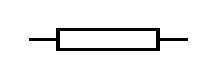
\begin{tikzpicture}
\draw[very thick] (0,0) -- ++(.37,0);
\draw[very thick] (1,0) node[rectangle,draw,minimum width=.5in,minimum height=.1in] {};
\draw[very thick] (1.65,0) -- ++(.37,0);
\end{tikzpicture}
};
\draw (1,-2) node (R3) {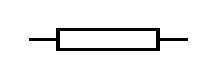
\begin{tikzpicture}
\draw[very thick] (0,0) -- ++(.37,0);
\draw[very thick] (1,0) node[rectangle,draw,minimum width=.5in,minimum height=.1in] {};
\draw[very thick] (1.65,0) -- ++(.37,0);
\end{tikzpicture}
};


\draw (R1) node[above=6pt] {$Z_{1}(s)$};
\draw (R2) node[above=6pt] {$Z_{2}(s)$};
\draw[very thick] (R1.180) |- (n1);
\draw[very thick] (R2.180) |- (n1);
\draw[very thick] (R1.0) |- (n2);
\draw[very thick] (R2.0) |- (n2);

\draw (R3) node[above=6pt] {$Z_{3}(s)$};
\draw (1,-2.75) node {$Z_{3}(s) = \frac{Z_{1}(s)Z_{2}(s)}{Z_{1}(s)+Z_{2}(s)}$};

%\draw (6.1,.75) node[above] {$+$};
%\draw (7,.75) node[above] {$X(s)$};
%\draw (7.9,.75) node[above] {$-$};

\end{tikzpicture}